\documentclass{article}
\usepackage{amssymb} 
\usepackage{amsmath, amsthm}
\usepackage{dsfont}
\usepackage{graphicx}
\usepackage{tikz}



\newtheorem{theorem}{Teorema}[section] 
\newtheorem{proposition}[theorem]{Proposizione} 
\newtheorem{corollary}[theorem]{Corollario}  
\newtheorem{lemma}[theorem]{Lemma}
\theoremstyle{definition}
\newtheorem{esercizio}{Esercizio}
\theoremstyle{definition}
\newtheorem{soluzione}{Soluzione}
\theoremstyle{definition}
\newtheorem{definition}[theorem]{Definizione}
\newtheorem{example}[theorem]{Esempio}

\theoremstyle{remark}
\newtheorem{remark}[theorem]{Osservazione}

\begin{document}

\section{Algebre e Algebre induttive}
\subsection{Introduzione e definizione}
\begin{definition}[Assiomi di Peano]
    \leavevmode\newline
    \begin{enumerate}
        \renewcommand{\labelenumi}{\Roman{enumi}.}
        \item $\varnothing  \in \mathbb{N}$
        \item  se $n\in\mathbb{N}\implies \sigma(n)\in\mathbb{N}$
        \item $\not\exists n\quad t.c.\quad \sigma(n)= \varnothing$
        \item $\forall m,n \quad \sigma(m)=\sigma(n)\implies n = m$
        \item $\forall S\subseteq \mathbb{N}$ (se $\varnothing \in S$ e $n\in S \implies \sigma(n)\in S)\implies S=\mathbb{N}$
    \end{enumerate}
\end{definition}
Il quinto assioma è equivalente all'induzione, ovvero: sia $P$ una proprietà su $\mathbb{N}$, se $P(0)$ e si assume sia vera fino ad $n$, quindi
$P(n)$ se si dimostra che $P(n+1)$ è vero allora $P$ è vera per ogni $n$. Attraverso questi assiomi abbiamo costruito la "struttura" dei numeri naturali che non è altro che un caso particolare di algebra.
La definizione di peano quindi è un modo per definire un'\textbf{algebra induttiva}. Le algebre sono degli insiemi dotati di operazioni
definite sugli elementi dell'insieme stesso, nel caso delle algebre eterogenee vengono coinvolti anche parametri esterni. Le operazioni definite in questi insiemi
hanno il codominio nell'insieme stesso, consideriamo ad esempio la seguente algebra:

\begin{example}
    Sia $A$ l'insieme dotato di un operazione $\gamma$ definita come segue:
    $$\gamma:  A\times K\to A $$
    dove $K$ è una collezione di elementi diversa da $A$. Anche l'operazione $\eta: K\to A$  che non prende elementi da $A$ può essere un'operazione valida.
\end{example}
\begin{definition}
    Un insieme $S$ si dice chiuso rispetto ad un'operazione $\gamma$ se:
    \begin{enumerate}
        \item $a\in S\implies\gamma(a)\in S$
        \item $a_1,a_2,\dots,a_k\in S\implies \gamma(a_1,a_2,\dots a_k)\in S$
        \item Preso $m\in M$ e $a_1,a_2\in S\implies \gamma(m,a_1,a_2)\in S$
    \end{enumerate}
    (nel (3) $m$ può essere un qualunque elemento di $M$ )
\end{definition}
\begin{definition}
    Un'algebra $(A,\gamma)$, dove $\gamma$ rappresenta una famiglia di operazioni $\{\gamma_i\}$, si dice induttiva quando:
    \begin{enumerate}
        \item Tutte le $\gamma_i$ sono iniettive.
        \item Le $\gamma_i$ hanno immagini disgiunte.
        \item $\forall S\subseteq A$ se $S$ è chiuso rispetto a tutte le  $\gamma_i$ allora $S=A$.
    \end{enumerate}
    L'insieme $A$ è chiamato \textit{insieme sottostante} all'algebra e rappresenta il codominio di ogni operazione $\gamma_i\in \gamma$.
\end{definition}
Quindi $\mathbb{N}$ è solo un caso particolare di algebra induttiva definita su gli interi positivi, dotata dell'operazione $\sigma$ e dell'operazione $\varnothing$.
Quest'ultima merità un piccolo approfondimento, infatti il terzo assioma di Peano impone che $\varnothing$ non sia immagine di alcun $\sigma(n)$, abbiamo quindi bisogno di definire un'operazione speciale
che mappa nello zero:

$$\varnothing: \mathds{1}\to\mathbb{N} $$
Dove $\mathds{1}$ denota l'insieme banale (o $\mathbb{N}^0$ ovvero un insieme composto da un solo elemento). La definizione di algebra induttiva ci serve per definire una collezione di oggetti in cui si esclude tutto ciò che non è
possibile costruire a partire dalle operazioni definite.
\begin{example}[Algebra di liste]
    Definiamo $L$ l'insieme delle liste ordinare di interi e una famiglia di operazioni $\gamma_L$ formata da due operazioni, $cons$, $empty$, diciamo che $(L,\gamma_L)$ è un'algebra induttiva. Definiamo $cons$ come l'operazione che dato un naturale e una lista, aggiunge quel numero in coda alla lista:
    $$cons(n,(n_1,\dots,n_q)) = (n,n_1,\dots,n_q)$$
    $empty$ invece è l'operazione con dominio in $\mathds{1}$ che mappa nella lista vuota $()$. Quindi $cons$ e $empty$ rispettano gli assiomi di algebra induttiva, in particolare: le immagini sono disgiunte, le operazioni sono iniettive e non esistono sotto-algebre chiuse per $cons$ e $empty$.
    Grazie alla struttura induttiva appena costruita possiamo  definire l'operazione $append$, che prende due liste e le unisce. Ecco un esempio di definizione ricorsiva:

    $$append((),l) = l$$
    $$append(cons(n,l),l') = cons(n,append(l,l'))\qquad\text{con $n\in\mathbb{N}$ e $l,l'\in L$}$$


\end{example}
\begin{example}(Booleani) sia $\mathbb{B} = \{True,False\}$ e siano $t,f$ due operazioni:
    $$ t:\mathds{1}\to\mathbb{B}$$
    $$ f:\mathds{1}\to\mathbb{B}$$
    Quindi $t(\mathds{1}) = True$ e $f(\mathds{1}) = False$, da questa definizione segue che  $(\mathbb{B},\{f,t\})$ è un algebra induttiva.
\end{example}
\begin{theorem}
    Un algebra induttiva è finita se e solo se  i costruttori hanno solo parametri esterni.
\end{theorem}
Un esempio banale  è $\mathbb{B}$ $( 1.8)$.
\subsection{Lemma di Lambek}
\subsubsection{Precisazione sulla notazione}
La segnatura algebrica delle operazioni di un'algebra è rappresentata da un'isieme $I$, di nomi di funzione e per ogni $i\in I$ corrisponde un $\alpha_i\ge 0$, che indica il numero di
parametri che l'operazione prende dall' insieme sottostante all' algebra, e un vettore $\mathbf{K_i}=(K_{i1},\dots,K_{iq})$, contente i domini da cui vengono presi i paramentri esterni per l'operazione,
quindi la dimensione del vettore  rappresenta il numero dei parametri esterni.
Due segnature di due algebre sono equivalenti se è possibile ottenere l'una dall'altra semplicemente scambiando gli insiemi sottostanti all'algebra nei singoli costruttori.
\begin{example}
    Consideriamo $(A,f_A)$ e $(B,f_B)$, con $f_A:A\times K \to A$ e \\$f_B:B\times K \to B$, le due algebre hanno la stessa segnatura perché è possibile ottenere $f_A$
        semplicemente sostituendo in $f_B$ $B$ con $A$. Quindi l'equivalenza di segnature è semplicemente un'equivalenza nella "forma" di ogni costruttore dell'algebra.
\end{example}
\begin{definition}  $h:(A,\gamma_A)\to(B,\gamma_B)$ è un omomorfismo di algebre se per ogni $ i\in I$
    $$h(\gamma_{A_i}(a_1,\dots a_{\alpha_i},k_1,\dots,k_{\beta_i})) = \gamma_{B_i}(h(a_1),\dots,h(a_{\alpha_i}),k_1,\dots, k_{\beta_i}). $$
    Un omomorfismo bigettivo è chiamato \textit{isomorfismo}.
\end{definition}
\begin{theorem}
    Siano $(A,\gamma_A)$ un'algebra induttiva e $(B,\gamma_B)$ un'algebra (non necessariamente induttiva), con operazioni con la
    stessa segnatura, allora esiste un unico omomorfismo  $h$:
    $$h:(A,\gamma_A)\to(B,\gamma_B)$$
\end{theorem}
\begin{example}
    Consideriamo l'algebra induttiva dei naturali e $(\mathbb{B},true,not)$, dove $not(true) = false$ e $not(false) = true$. Per il teorema $(1.10)$ esiste un unico omomorfismo di algebre $h:\mathbb{N}\to\mathbb{B}$ definito
    come :
    $$h(\varnothing) = True$$
    $$h(\sigma(n)) = not(h(n))$$
\end{example}
\begin{lemma}[Lambek] Due algebre induttive con stessa segnatura sono isomorfe.
\end{lemma}
\begin{proof}[Dimostrazione]

    Siano $A$ e $B$ due algebre induttive, per $\mathbf{(1.11)}$ esiste un unico omomorfismo $h:A\to B$ e viceversa $h':B\to A$.
    $$A\xrightarrow{h} B\xrightarrow{h'} A$$
    Consiederiamo ora $h'\circ h: A\to A$, ovviamente la composizione di due omomorfismi è anch'esso un omomorfismo, per esempio la funzione identità $Id: A\to A$ è un omomorfismo
    da $A$ in $A$. Ricordiamo che dal precedente teorema sappiamo che tale omomorfismo è unico, segue che $h'\circ h = Id$ e quindi $h' = h^{-1}$.
\end{proof}

Affinchè sia presente un isomorfismo è necessaria una bigezione tra gli insiemi sottostanti all'algebra, ma quest'ultima non è sufficiente a garantire l'uguaglianza nella struttura, infatti
è necessario che anche le segnature siano le stesse.
\begin{example} Prendiamo il caso di due insiemi di interi positivi $\mathbb{N}$ e $\mathbb{N}_*:=\{0,1,\dots,*\}$, esiste certamente una mappa biettiva tra i due insiemi, ma non è possibile stabilire un isomorfismo tra le due algebre, in quanto la segnatura delle rispettive
    famiglie di operazioni sarà diversa.
\end{example}
\subsection{Algebra induttiva di alberi binari}
\begin{theorem}
    Ogni albero binario con $n$ foglie ha $2n-1$ nodi.
\end{theorem}

Per dimosteare questo teorema possiamo utilizzare l'induzione completa, ma ai fini del nostro studio, risulta più istruttivo utilizzare l'\textit{induzione strutturale} su un'algebra induttiva di alberi binari.
Sia $B_{tree}$ l'insieme di tutti gli alberi binari finiti. Dotiamo $B_{tree}$ di due costruttori:
\begin{itemize}
    \item [-] $root : \mathds{1}\to B_{tree}$, un costruttore di base che mappa nell'albero binario formato da un solo nodo.
    \item [-] $branch: B_{tree}\times B_{tree} \to B_{tree}$, un costruttore che unisce due alberi binari, aggiungendo una radice e attaccando i due alberi alla radice, uno come sottoalbero destro e uno come sotto albero sinistro.
\end{itemize}
Le due operazioni rispettano gli assiomi di algebra
induttiva, quindi \\$(B_{tree},root,branch)$ è un'algebra induttiva.
    Possiamo ora applicare l'induzione sull'algebra di alberi binari, modificando l'induzione sui naturali:
    $$ \frac{P(0)\quad P(n)\implies P(\sigma(n))}{\forall n\quad P(n)}\to \frac{P(root)\quad P(t_1),P(t_2)\implies P(branch(t_1,t_2))}{\forall t \quad P(t)}$$

    \begin{proof}[\textbf{Dimostrazione (1.14)}]Il caso base è banale infatti $|root| = 2(1)-1 = 1$. Applichiamo il passo induttivo e dimostriamo che, dati
        $t_1$ e $t_2$ due alberi binari con $|t_1| =2n_1-1$, $|t_2| = 2n_2-1$,  allora $|branch(t_1,t_2)| = 2n_1-1 + 2n_2 -1 +1 = 2(n_1+n_2)-1$.
    \end{proof}

    Durante la costruzione dell'algebra abbiamo specificato la presenza  solo di alberi finiti, in quanto un elemento in sé infinito (in questo caso un albero), violerebbe gli assiomi di algebra induttiva. Quindi le collezioni di elementi con operazioni che contengono elementi di questo tipo
    vengono chiamate algebre \textit{co-induttive}.

    \subsection{Esercizi}
    \begin{definition}
        Un costruttore è  ogni $\gamma_i$ appartenente alla famiglia di operazioni di un algebra $(A,\gamma)$. Un costruttore di base non ha parametri presi dall'insieme sottostante all'algebra, ovvero $\alpha_i = 0$.
    \end{definition}
    \begin{esercizio}
        Dimostrare che ogni algebra induttiva non vuota ha almeno un
        costruttore base.
    \end{esercizio}
    \begin{proof}[\textbf{Soluzione}]Sia $(A,\boldsymbol{\gamma})$, con $\boldsymbol{\gamma} = (\gamma_1,\dots, \gamma_k)$, un'algebra induttiva.
        Consideriamo $\varnothing \subsetneq A$, questo è chiaramente chiuso per ogni $\gamma_i$ che non sia di base, quindi se supponiamo
        che non esistano  in $\boldsymbol{\gamma}$ costruttori di base allora $(\varnothing,\boldsymbol{\gamma})$ è un algebra induttiva, andando in
        contrapposizione con il terzo assioma. Segue l'esistenza di almeno un costruttore base.
    \end{proof}
    \begin{esercizio}
        Dimostrare che ogni algebra induttiva non vuota con un
        costruttore non base è necessariamente infinita.
    \end{esercizio}
    \begin{proof}[\textbf{Soluzione}] Sia $b\in A$  l'elemento mappato dal costruttore di base $\beta$ (di cui abbiamo
        verificato l'esistenza nell'esercizio sopra), se $A$ è dotato anche di un costruttore
        non di base $\gamma$, allora $\gamma(b) = a_1$, $\gamma(a_1) = a_2$ e così via senza mai giungere ad una fine.
        Infatti se volessimo provare a chiudere la sequenza, ad esempio proprio con $\gamma(a_n)=b$, otterremmo delle
        immagini di $\gamma$ e $\beta$ non disgiunte contraddicendo gli assiomi di algebra induttiva, segue la non finitezza di $A$.
    \end{proof}
    \begin{esercizio}
        Consideriamo alberi binari con nodi etichettati da numeri
        naturali. Eccone uno:
        \begin{center}


            \tikzset{every picture/.style={line width=0.75pt}} %set default line width to 0.75pt        

            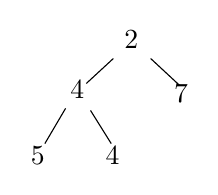
\begin{tikzpicture}[x=0.75pt,y=0.75pt,yscale=-1,xscale=1]
                %uncomment if require: \path (0,300); %set diagram left start at 0, and has height of 300

                %Straight Lines [id:da07036281093773067] 
                \draw    (219,129) -- (209,146) ;
                %Straight Lines [id:da529798846812493] 
                \draw    (241,146) -- (231,130) ;
                %Straight Lines [id:da7883803887618286] 
                \draw    (242,105) -- (229,117) ;
                %Straight Lines [id:da034539223291089605] 
                \draw    (260,105) -- (274,118) ;

                % Text Node
                \draw (246,90.4) node [anchor=north west][inner sep=0.75pt]    {$2$};
                % Text Node
                \draw (220,114.4) node [anchor=north west][inner sep=0.75pt]    {$4$};
                % Text Node
                \draw (201,146.4) node [anchor=north west][inner sep=0.75pt]    {$5$};
                % Text Node
                \draw (270,116.4) node [anchor=north west][inner sep=0.75pt]    {$7$};
                % Text Node
                \draw (237,146.4) node [anchor=north west][inner sep=0.75pt]    {$4$};


            \end{tikzpicture}

        \end{center}
        Definire l’algebra induttiva $BN$-$trees$ di questi alberi.Definire un’algebra di
        uguale segnatura sull’insieme $S$ delle sequenze finite di numeri naturali in modo
        che la funzione $f : BN\text{-}trees\to S$ che associa a ciascun albero la sequenza di
        etichette ottenuta con una visita depth-first sia un omomorfismo. Applicando $f$
        all’albero dell’esempio, ci aspettiamo di ottenere la sequenza ⟨2,4,5,4,7⟩.
        \begin{proof}[\textbf{Soluzione}]
            Definiamo un'estensione delle operazioni create in precedenza per l'algebra di $B_{tree}$:
            $$branch^*: BN\text{-}tree\times BN\text{-}tree\times \mathbb{N}\to BN\text{-}tree,$$
            $$root^*: \mathbb{N}\to BN\text{-}tree.$$
            $branch^*$ prende in input due alberi e un intero che etichetterà la radice; $root^*$ invece prende un
            intero $n$ e crea la radice etichettata con $n$. In modo del tutto analogo definiamo sull'insieme $S$ l'operazione
            di concatenazione di due serie numeriche $s_1, s_2$ di lunghezza dispari che restituisca una serie dispari:
            $$\mathcal{C}:S\times S\times \mathbb{N}\to S$$
            $$\mathcal{C}(s,s',n)\mapsto \langle n,s_1,\dots,s_k,s_1',\dots,s_q'\rangle$$
            \newpage

            $$\Lambda : \mathbb{N}\to S$$
            $$\Lambda(n)\mapsto \langle n\rangle$$
            Come conseguenza del \textit{lemma di Lambek} $(1.12)$ esiste  ed è unico l' omomorfismo $f:B\text{-}tree\to S$.
            Consideriamo la sequenza $s = \langle s_1\dots s_k\rangle$ generata visitando con una $DFS$ l'albero $t\in B\text{-}tree$,
            quindi $f(t) = s$. In particolare $f$ è un omomorfismo di algebre
            \begin{equation}
                f(branch(t_1,t_2,a)) = \mathcal{C}(f(t_1),f(t_2),a)
            \end{equation}
            \begin{equation}
                f(root^*(n)) = \Lambda(n)
            \end{equation}
            La $(1)$ è giustificata dal fatto che la  $depth$-$first$ visita l'albero  da  sinistra a destra, e quindi la sequenza
            risultante avrà inizialmente $a$ (la radice del nuovo albero prodotto da $branch$) $f(t_1)$  ed infine $f(t_2)$.
        \end{proof}
    \end{esercizio}

    \section{Linguaggi di espressioni}
    \begin{definition}
        Sia $L$ un linguaggio, un insieme di stringhe generate dalla grammatica
        $$M,N ::= 1|2|...|M+N|M*N.$$
    \end{definition}
    \begin{example}
        Ad esempio $3+5$,$3*5$ e $4*5+2$ sono delle espressioni di $L$.
    \end{example}
    Introduciamo la funzione $eval:L\to \mathbb{N}$, per valutare la sintassi delle espressioni:
    $$eval(n) = n$$
    $$eval(M+N) = eval(M) + eval(N)$$
    $$eval(M*N) = eval(M) * eval(N)$$
    Possiamo definire la funzione $eval$ per casi, ma non è stato definito un modo univoco per
    valutare delle espressioni come $\mathbf{"5+4*3"}$, viene svolta prima la $*$ o il $+$ ?\\ Per come è stato costruito il linguaggio $L$ dotato delle operazioni $+$ e $*$ non può essere un'algebra induttiva. Per disambiguare queste espressioni dobbiamo riformulare  il linguaggio in modo da renderlo un algebra induttiva.
    Per iniziare dobbiamo dare una rappresentazione di senso univoco alle espressioni del tipo $\mathbf{"5+4*3"}$, scriviamo più formalemente:
    $$\mathbf{1}:\mathds{1}\to L$$
    $$\mathbf{2}:\mathds{1}\to L$$
    $$\vdots$$
    $$times:L\times L\to L$$
    $$plus :L\times L\to L$$
    Allora $(L,\mathbf{1},\mathbf{2},\dots,times,plus)$ è un'algebra induttiva.
    \newpage
    Quindi l'$eval$ di  $\mathbf{"5+4*3"}$ può essere:
$$eval(\mathbf{"5+4*3"}) = \left\{ \begin{array}{cl}
        eval(times(plus(\mathbf{5}(\epsilon),\mathbf{4}(\epsilon)),\mathbf{3}(\epsilon))) \\
        eval(plus(\mathbf{5}(\epsilon),times(\mathbf{4}(\epsilon),\mathbf{3}(\epsilon))))
    \end{array}\right.$$
Pur essendo quella definita sopra la notazione corretta, utilizzarla per le nostre valutazioni risulterebbe
inutilmente complessa, per questo motivo faremo uso della classica notazione con le parentesi per definire le precedenze.
Ad esempio $$plus(\mathbf{5}(\epsilon),times(\mathbf{4}(\epsilon),\mathbf{3}(\epsilon))) = 5+(4*3).$$
\end{document}
